\section{The physics floor}\label{sec:floor}
\sectionstate{partial}{toy closure, WFT \S12 (\texttt{18\_toy\_closure.py}, R\&D model)}
\intent{What limits the angle once the bias is gone: electronics contribute 0.02\textdegree; $\sim$1\textdegree{} comes from
the 0.3\,mm jitter of the charge centroid (diffusion). The floor is physics, not readout.}
\analysis{R6}{re-run the toy on the production model and the r06 kernel}
\begin{figure}[t]
  \centering
  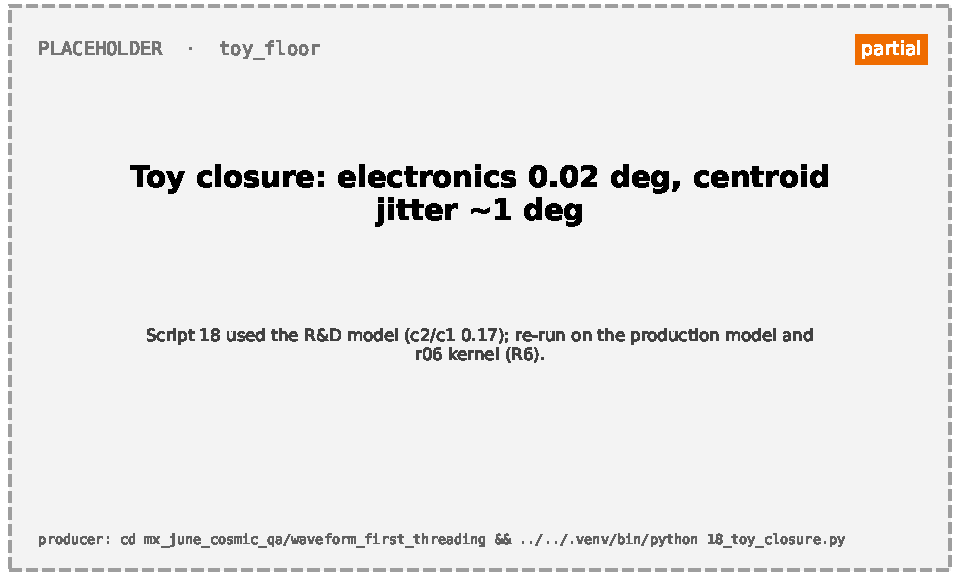
\includegraphics[width=0.7\linewidth]{toy_floor}
  \caption{\tbw{Toy closure: contributions to the angular resolution.}}
  \label{fig:toy_floor}
\end{figure}
